\subsection{Monte Carlo Calibration}

The MC calibration is based on the simulation and corrects the energy of the reconstructed jets such that it is equal on average to the energy of the generated MC particle jets. Simulated QCD events are generated with {\sc PYTHIA}6.4.22~\cite{PYTHIA}, tune Z2 (the {\sc Z2} tune is identical to the {\sc Z1} tune described in~\cite{D6T} except that {\sc Z2} uses the CTEQ6L PDF, while {\sc Z1} uses CTEQ5L) and processed through the CMS detector simulation, based on {\sc GEANT4}~\cite{GEANT4}. The jet reconstruction is identical to the one applied to the data. Each reconstructed jet is spatially matched in the $\eta-\phi$ space with a MC particle jet by requiring $\Delta R<0.25$. In each bin of the MC particle transverse momentum $\pt^{gen}$, the response variable $\mathcal{R}=\pt^{reco}/\pt^{gen}$ and the detector jet $\pt^{reco}$ are recorded. The average correction in each bin is defined as the inverse of the average response $C_\text{MC}(\pt^{reco})=\frac{1}{<\mathcal{R}>}$, and is expressed as a function of the average detector jet \pt $<\pt^{reco}>$. Figure~\ref{fig:mctruthVsEta} shows the MC jet energy correction factor for the three jet types, vs. $\eta$, for different corrected jet \pt values. Figure~\ref{fig:mctruthVsPt} shows the average correction in $|\eta|<1.3$, as a function of the corrected jet \pt.

Calorimeter jets require a large correction factor due to the non-linear response of the CMS calorimeters. The structures observed at $|\eta|\sim 1.3$ are due to the barrel-endcap boundary and to the tracker material budget, which is maximum in this region. The fast drop observed in the endcap region $1.3<|\eta|<3.0$ is due to the fact that the jet energy response depends on energy rather than on jet \pt. For higher values of $|\eta|$ more energy corresponds to a fixed \pt value $E\approx\pt\cdot\cosh(\eta)$, which means that the jet response is higher and the required correction factor is smaller. The structure observed at $|\eta|\sim 3.0$ coincides with the boundary between the endcap and the forward calorimeters. Finally, in the region $|\eta|>4.0$, the jet energy response is lower because parts of the jets pointing toward this region extend beyond the forward calorimeter acceptance.

The track-based jet types (JPT and PF) require much smaller correction factors because the charged component of the jet shower is measured accurately in the CMS tracker which extends up to $|\eta|=2.4$. The fast rise of the correction factor for JPT jets in the region $2.0<|\eta|<2.5$ is explained by the fact that part of the jets lying in this region extends beyond the tracker coverage. For PF jets, the transition beyond the tracker acceptance is smoother because the PF candidates, which are input to the clustering of PF jets, are individually calibrated prior to the clustering. While both PF jets and JPT jets exploit the tracker measurements, the JPT jets require lower correction in the region $|\eta|<2.0$ because the tracker inefficiency is explicitly corrected for by the JPT algorithm.
In the forward region ($|\eta|>3.0$) all three jet types converge to simple calorimetric objects and therefore require almost identical corrections.

\begin{figure}[ht!]
  \begin{center}
    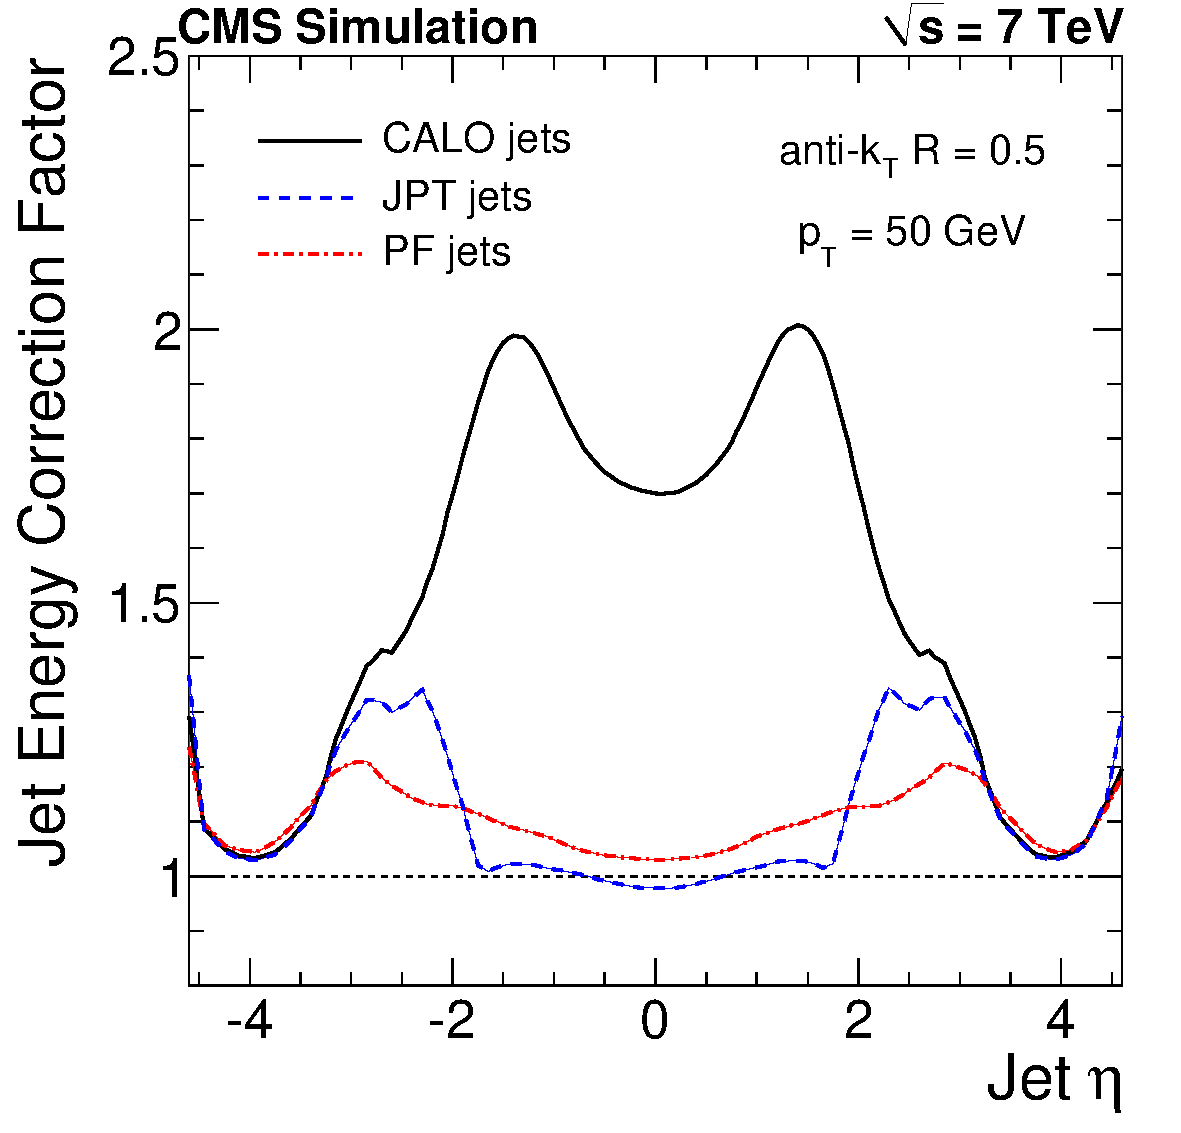
\includegraphics[width=0.45\textwidth]{Figures/JEC/JEC_MCtruth_vs_Eta_CorPt50}
    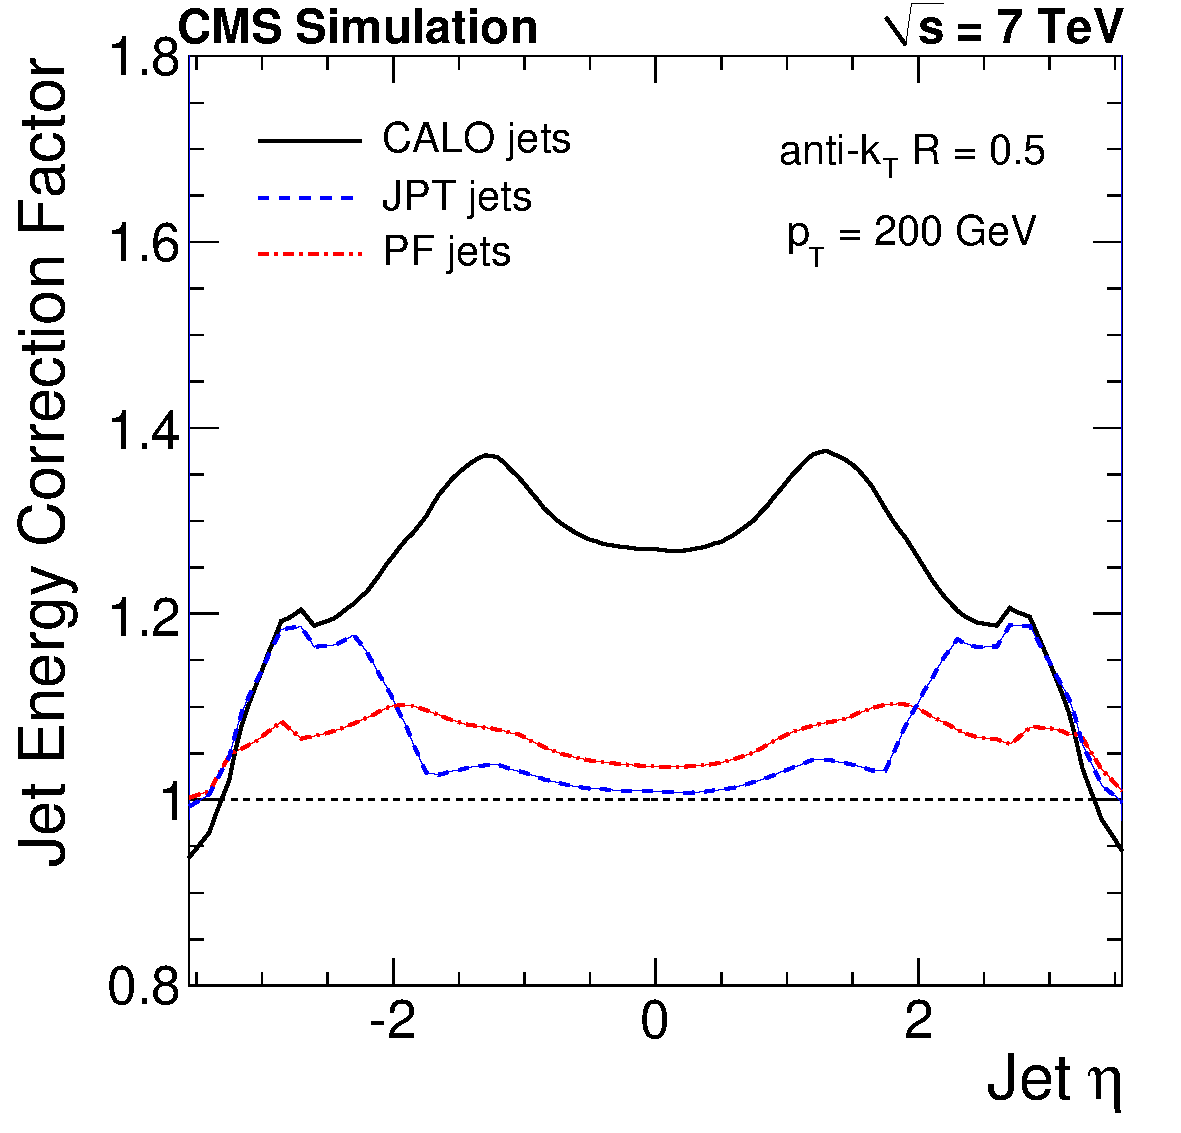
\includegraphics[width=0.45\textwidth]{Figures/JEC/JEC_MCtruth_vs_Eta_CorPt200}
    \caption{Monte Carlo jet-energy-correction factors for the different jet types, as a function of jet $\eta$. Left: correction factor required to get a corrected jet $\pt=50\GeV$. Right: correction factor required to get a corrected jet $\pt=200\GeV$.}
    \label{fig:mctruthVsEta}
  \end{center}
\end{figure}

\begin{figure}[ht!]
  \begin{center}
    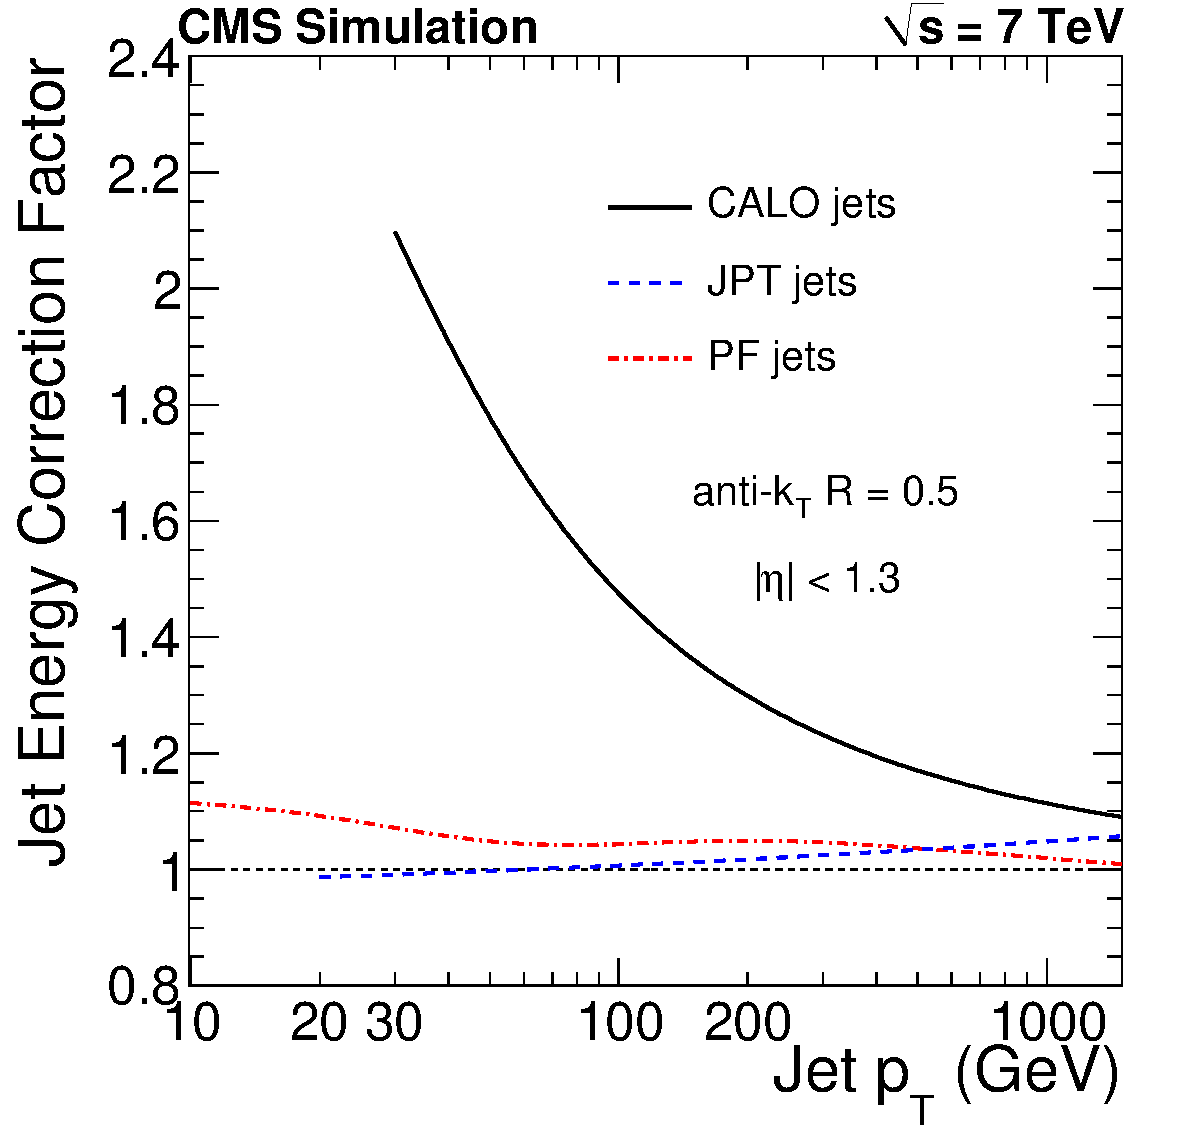
\includegraphics[width=0.45\textwidth]{Figures/JEC/JEC_MCtruth_vs_CorPt_Barrel}
    \caption{Monte Carlo jet-energy-correction factors for the different jet types, as a function of jet \pt.}
    \label{fig:mctruthVsPt}
  \end{center}
\end{figure}

The default MC calibration is derived from the QCD sample and corresponds to a jet flavour composition enriched in low-\pt gluon jets. The jet energy response and resolution depend on the fragmentation properties of the initial parton: gluons and heavy-flavour quarks tend to produce more particles with a softer energy spectrum than light quarks. The investigation of the jet energy response of the various flavour types, for the different jet reconstruction techniques, is done with MC matching between the generated particle jet and the reconstructed jet. For each MC particle jet, the corresponding parton is found by spatial matching in the $\eta-\phi$ space. Figure~\ref{fig:flavor} shows the response of each flavour type (gluon, b-quark, c-quark, uds-quark), as predicted by {\sc PYTHIA6} (Z2 tune), in the region $|\eta|<1.3$, normalized to the average response in the QCD flavour mixture. The QCD flavour composition varies significantly with jet \pt, being dominated by gluon jets at low \pt and by quark jets at high \pt. Calorimeter jets show strong dependence on the flavour type with differences up to 10\%. This is attributed to the non-linear single-particle response in the calorimeters. For the track-based reconstructed jets, the flavour dependence is significantly reduced and not larger than 5\% and 3\% for JPT and PF jets respectively. The ability to measure precisely the charged particle momenta in the tracker reduces the contribution of calorimetry at low jet \pt. In all jet types, the jets originated from a light quark (u/d/s) have a systematically higher response than those from the other flavours, which is attributed to the harder spectrum of the particles that are produced in the fragmentation process. For comparison, Fig.~\ref{fig:flavor_herwigpythia} shows the flavour dependent response ratio of a different fragmentation model ({\sc Herwig++}) with respect to {\sc PYTHIA6}. 

\begin{figure}[ht!]
  \begin{center}
    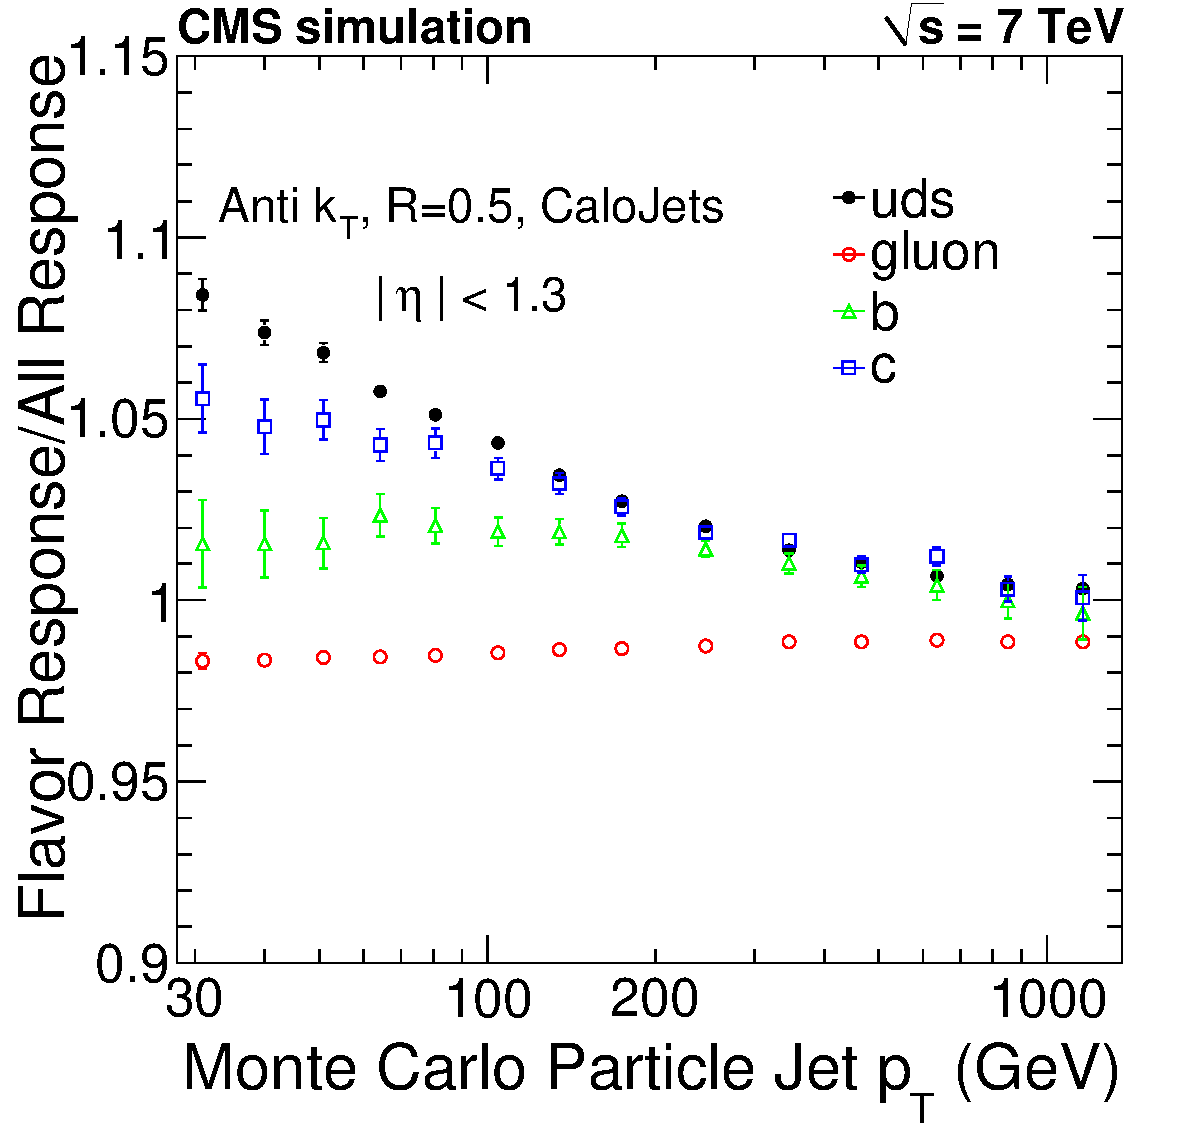
\includegraphics[width=0.32\textwidth]{Figures/JEC/ak5calo_FlavorRsp}
    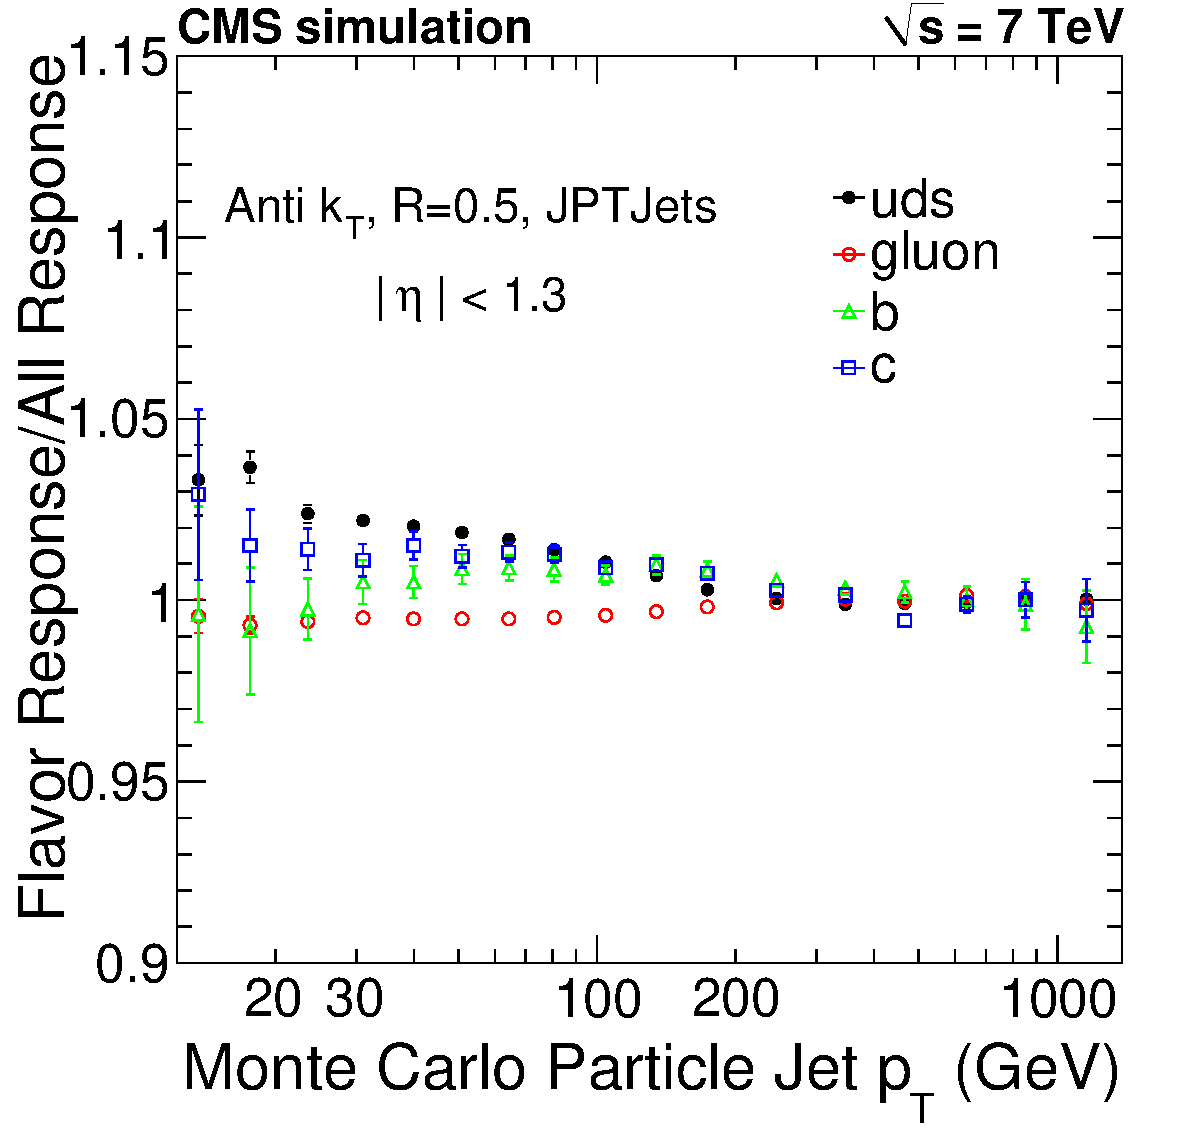
\includegraphics[width=0.32\textwidth]{Figures/JEC/ak5jpt_FlavorRsp}
    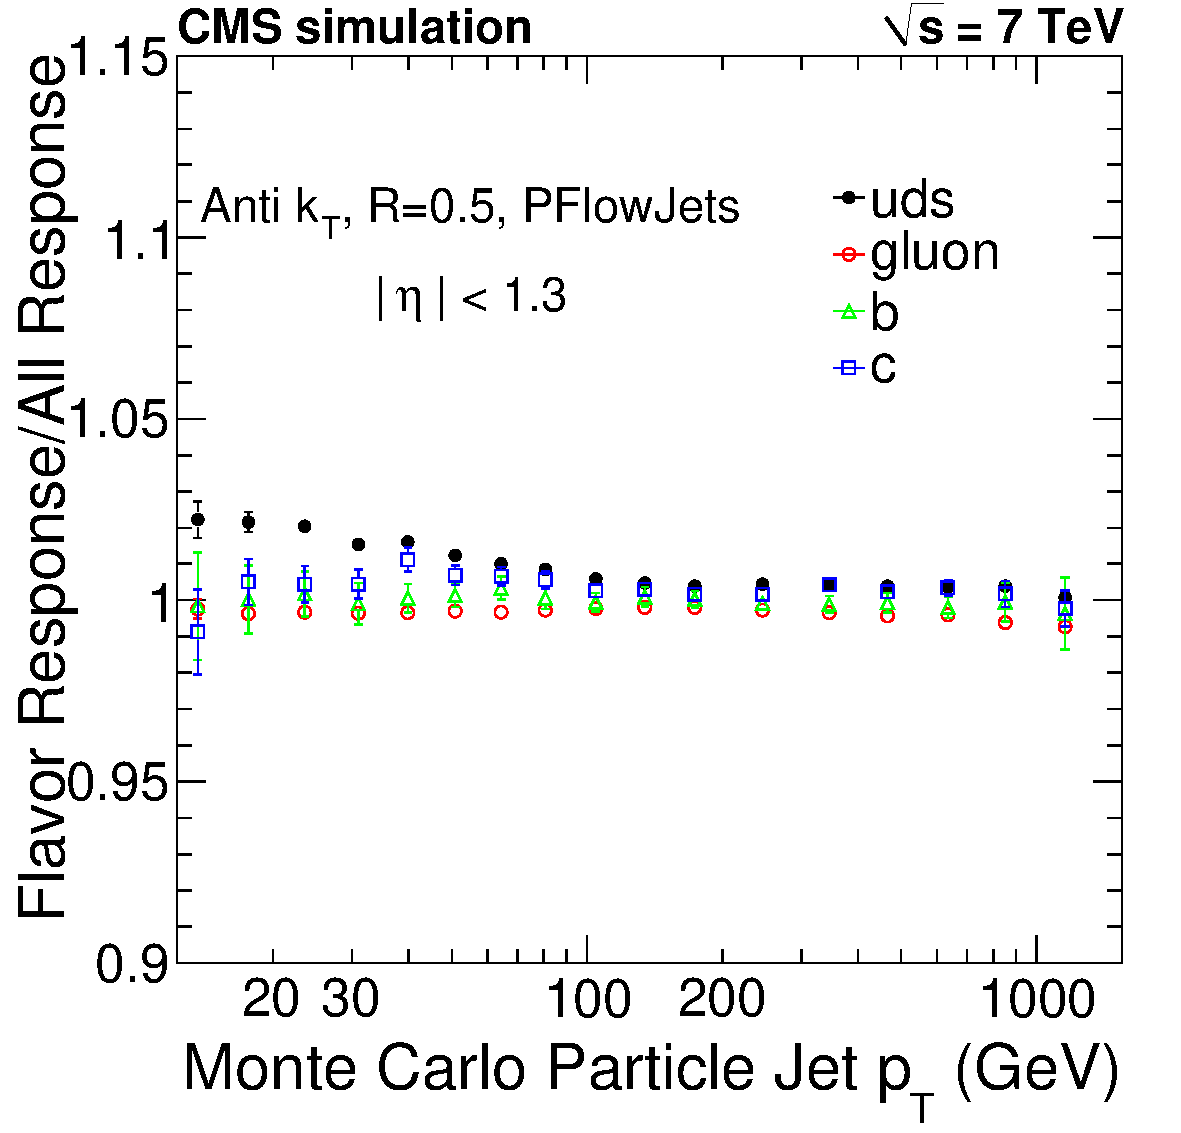
\includegraphics[width=0.32\textwidth]{Figures/JEC/ak5pf_FlavorRsp}
    \caption{Simulated jet energy response, in {\sc PYTHIA6} Z2 tune, of different jet flavours normalized to the response of the QCD flavour mixture, as a function of the true particle jet \pt, in the region $|\eta|<1.3$ for the three jet types.}
    \label{fig:flavor}
  \end{center}
\end{figure}

\begin{figure}[ht!]
  \begin{center}
    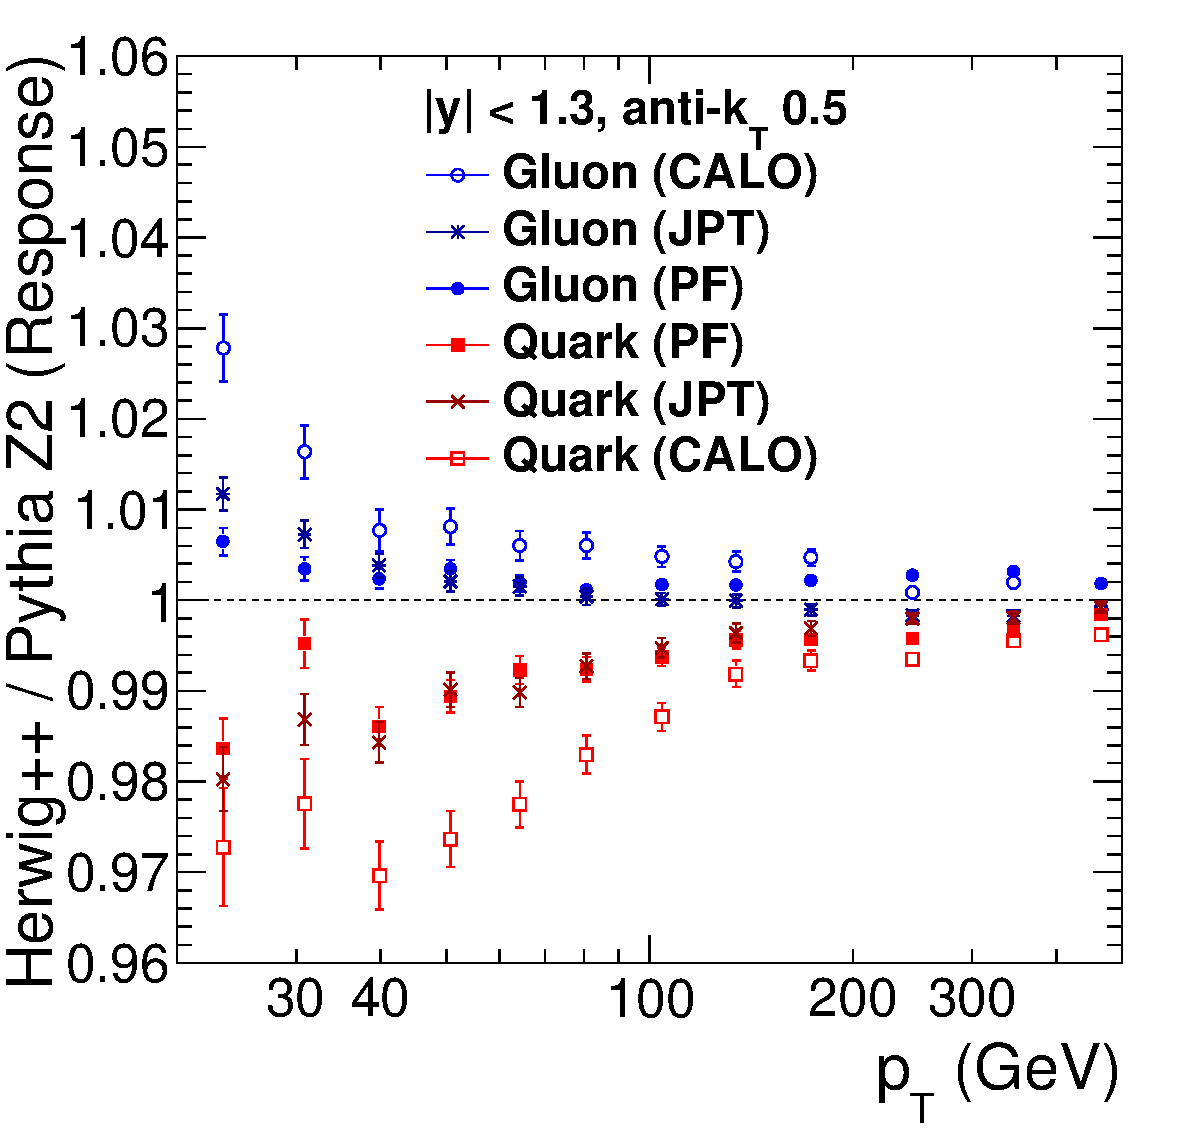
\includegraphics[width=0.45\textwidth]{Figures/JEC/flavor_herwigpythia}
    \caption{Response ratio predicted by {\sc Herwig++} and {\sc PYTHIA6} for jets originated by light quarks (uds) and gluons for the various jet types.}
    \label{fig:flavor_herwigpythia}
  \end{center}
\end{figure}
